\documentclass[11pt,a4paper]{article}

% Rigtig god opave.
%
% ret fejlene i:
% · 1.2.3u
%
% lav:
% · extraopgaven punkt 5

\usepackage[utf8]{inputenc}
\usepackage{a4wide}
\usepackage{amsmath,amssymb}
\usepackage{boxproof}
\usepackage{daymonthyear}
\usepackage{float} % for the H placement identifier
\usepackage{graphicx}
\usepackage{tikz}
\usepackage{tabu}
\usepackage{xcolor}

%===== SETTINGS =====%

\def\meta#1{\mbox{$\langle\hbox{#1}\rangle$}}
\def\macrowitharg#1#2{{\tt\string#1\bra\meta{#2}\ket}}

{\escapechar-1 \xdef\bra{\string\{}\xdef\ket{\string\}}}

\def\intro#1{{#1}{\cal I}}
\def\elim#1{{#1}{\cal E}}

\showboxbreadth 999
\showboxdepth 999
\tracingoutput 1

\let\imp\to
\def\elim#1{{{#1}{\cal E}}}
\def\intro#1{{{#1}{\cal I}}}
\def\lt{<}
\def\eqdef{=}
\def\eps{\mathrel{\epsilon}}
\def\biimplies{\leftrightarrow}
\def\flt#1{\mathrel{{#1}^\flat}}
\def\setof#1{{\left\{{#1}\right\}}}
\let\implies\to
\def\KK{{\mathsf K}}
\let\squashmuskip\relax

%===== META DATA =====%

\title
{
{\Large Logic in Computer Science}\\
Assignment 2
}
\author
{
	Casper B. Hansen\\
	University of Copenhagen\\
	Department of Computer Science\\
	{\tt fvx507@alumni.ku.dk}
}
\date{\today}

%===== DOCUMENT =====%

\begin{document}

\maketitle

% For Exercise 1.2 1rs 3qu formal errors will not be tolerated

\section*{1.2.1 \mdseries For the sequents below, show which ones are valid and which ones aren't.}
% using natural deduction
\subsection*{(r) \mdseries $p \imp q \land r \vdash (p \imp q) \land (p \imp r)$}
\begin{proofbox}
	\lbl{1} \: p \imp q \land r 					\=\mbox{premise} \\
	\[
	\lbl{2} \: p 									\=\mbox{assumption} \\
	\lbl{3} \: q \land r 							\=\elim\imp(\ref{1}, \ref{2}) \\
	\lbl{4} \: q 									\=\elim\land_1(\ref{3}) \\
	\]
	\lbl{5} \: p \imp q 							\=\intro\imp(2-4) \\
	\[
	\lbl{6} \: p 									\=\mbox{assumption} \\
	\lbl{7} \: q \land r 							\=\elim\imp(\ref{1}, \ref{6}) \\
	\lbl{8} \: r 									\=\elim\land_2(\ref{7}) \\
	\]
	\lbl{9} \: p \imp r 							\=\intro\imp(6-8) \\
	\lbl{10} \: (p \imp q) \land (p \imp r) 		\=\intro\land(5, 9) \\
\end{proofbox}

\subsection*{(s) \mdseries $(p \imp q) \land (p \imp r) \vdash p \imp q \land r$}
\begin{proofbox}
	\lbl{1} \: (p \imp q) \land (p \imp r) 			\=\mbox{premise} \\
	\lbl{2} \: p \imp q 							\=\elim\land_1(\ref{1}) \\
	\lbl{3} \: p \imp r 							\=\elim\land_2(\ref{1}) \\
	\[
	\lbl{4} \: p 									\=\mbox{assumption} \\
	\lbl{5} \: q 									\=\elim\imp(\ref{2}, \ref{4}) \\
	\lbl{6} \: r 									\=\elim\imp(\ref{3}, \ref{4}) \\
	\lbl{7} \: q \land r 							\=\intro\land(\ref{5}, \ref{6}) \\
	\]
	\lbl{8} \: p \imp q \land r 					\=\intro\imp(4-7) \\
\end{proofbox}

\section*{1.2.3 \mdseries Prove the validity of the sequents below.}
% using natural deduction
\subsection*{(q) \mdseries $\vdash (p \imp q) \lor (q \imp r)$ using {\tt LEM}}
\begin{proofbox}
	\lbl{1} \: q \lor \neg q						\=\mbox{\tt LEM} \\
	\[
	\lbl{2} \: q 									\=\mbox{assumption} \\
	\[
	\lbl{3} \: p 									\=\mbox{assumption} \\
	\lbl{4} \: q 									\=\mbox{copy(\ref{2})} \\
	\]
	\lbl{5} \: p \imp q 							\=\intro\imp(3-4) \\
	\lbl{6} \: (p \imp q) \lor (q \imp r) 			\=\intro\lor_1(5) \\
	\]
	\[
	\lbl{7} \: \neg q								\=\mbox{assumption} \\
	\[
	\lbl{8} \: q 									\=\mbox{assumption} \\
	\lbl{9} \: \neg q 								\=\mbox{copy(\ref{7})} \\
	\lbl{10} \: \bot 								\=\elim\neg(\ref{8}, \ref{9}) \\
	\lbl{11} \: r 									\=\elim\bot(\ref{10}) \\
	\]
	\lbl{12} \: q \imp r 							\=\intro\imp(8-11) \\
	\lbl{13} \: (p \imp q) \lor (q \imp r) 			\=\intro\lor_2(\ref{12}) \\
	\]
	\lbl{14} \: (p \imp q) \lor (q \imp r)			\=\elim\lor(2-6, 8-13) \\
\end{proofbox}

\subsection*{(u) \mdseries $(s \imp p) \lor (t \imp q) \vdash (s \imp q) \lor (t \imp p)$}
\begin{proofbox}
	\lbl{1} \: (s \imp p) \lor (t \imp q) 			\=\mbox{premise} \\
	\[
	\lbl{2} \: s \imp p 							\=\mbox{assumption} \\
	\lbl{3} \: s \lor \neg s 						\=\mbox{\tt LEM} \\
	\[
	\lbl{4} \: s 									\=\mbox{assumption} \\
	\[
	\lbl{5} \: t 									\=\mbox{assumption} \\
	\lbl{6} \: p 									\=\elim\imp(\ref{2}, \ref{4}) \\
	\]
	\lbl{7} \: t \imp p 							\=\intro\imp(5-6) \\
	\lbl{8} \: (s \imp q) \lor (t \imp p)	 		\=\intro\lor_2(7) \\
	\]
	\[
	\lbl{9} \: \neg s 								\=\mbox{assumption} \\
	\[
	\lbl{10} \: s 									\=\mbox{assumption} \\
	\lbl{11} \: \bot 								\=\intro\neg(\ref{9}, \ref{10})\\
	\lbl{12} \: q 									\=\elim\neg(\ref{11}) \\
	\]
	\lbl{13} \: s \imp q 							\=\intro\imp(10-12) \\
	\lbl{14} \: (s \imp q) \lor (t \imp p) 			\=\intro\lor_1(7) \\
	\]
	\lbl{15} \: (s \imp q) \lor (t \imp p) 			\=\elim\lor(\ref{3}, 4-8, 9-14) \\
	\]
%
	\[
	\lbl{16} \: t \imp q 							\=\mbox{assumption} \\
	\lbl{17} \: t \lor \neg t 						\=\mbox{\tt LEM} \\
	\[
	\lbl{18} \: t 									\=\mbox{assumption} \\
	\[
	\lbl{19} \: s 									\=\mbox{assumption} \\
	\lbl{20} \: q 									\=\elim\imp(\ref{16}, \ref{18}) \\
	\]
	\lbl{21} \: s \imp q 							\=\intro\imp(19-20) \\
	\lbl{22} \: (s \imp q) \lor (t \imp p)	 		\=\intro\lor_1(21) \\
	\]
	\[
	\lbl{23} \: \neg t 								\=\mbox{assumption} \\
	\[
	\lbl{24} \: t 									\=\mbox{assumption} \\
	\lbl{25} \: \bot 								\=\intro\neg(\ref{23}, \ref{24}) \\
	\lbl{26} \: p									\=\elim\neg(\ref{25}) \\
	\]
	\lbl{27} \: t \imp p 							\=\intro\imp(24-26) \\
	\lbl{28} \: (s \imp q) \lor (t \imp p) 			\=\intro\lor_2(27) \\
	\]
	\lbl{29} \: (s \imp q) \lor (t \imp p) 			\=\elim\lor(\ref{16}, 18-22, 23-28) \\
	\]
	\lbl{28} \: ((s \imp p) \lor (t \imp q)) \imp ((s \imp q) \lor (t \imp p))
	\=\intro\imp(\ref{1}-29) \\
\end{proofbox}

\newpage
\section*{1.4.17 \mdseries Does $\models \phi$ hold for the $\phi$ below? Please justify your answer.}
\subsection*{(a) \mdseries $(p \imp q) \lor (q \imp r)$}
For this to be invalid, we would need to have both implications to evaluate to {\tt F}, for the $\lor$-expression to become {\tt F} as well. From this we can choose the cases that does indeed apply under these premises.
\begin{center}
	\begin{tabu}{ccccc|c}
		$p$ & $q$ & $r$ & $p \imp q$ & $q \imp r$ & $(p \imp q) \lor (q \imp r)$ \\ \hline
		\color{red} {\tt F} & \color{red} {\tt F} & \color{red} {\tt F} & \color{red} {\tt T} & \color{red} {\tt T} & \color{red} {\tt T} \\
		\color{red} {\tt F} & \color{red} {\tt F} & \color{red} {\tt T} & \color{red} {\tt T} & \color{red} {\tt T} & \color{red} {\tt T} \\
		\color{red} {\tt F} & \color{red} {\tt T} & {\tt F} & \color{red} {\tt T} & {\tt F} & \color{red} {\tt T} \\
		\color{red} {\tt F} & \color{red} {\tt T} & \color{red} {\tt T} & \color{red} {\tt T} & \color{red} {\tt T} & \color{red} {\tt T} \\
		{\tt T} & \color{red} {\tt F} & \color{red} {\tt F} & {\tt F} & \color{red} {\tt T} & \color{red} {\tt T} \\
		{\tt T} & \color{red} {\tt F} & \color{red} {\tt T} & {\tt F} & \color{red} {\tt T} & \color{red} {\tt T} \\
		\color{red} {\tt T} & \color{red} {\tt T} & {\tt F} & \color{red} {\tt T} & {\tt F} & \color{red} {\tt T} \\
		\color{red} {\tt T} & \color{red} {\tt T} & \color{red} {\tt T} & \color{red} {\tt T} & \color{red} {\tt T} & \color{red} {\tt T} \\
	\end{tabu}
\end{center}
Marked by red, we see the valuations that cause the expression to become {\tt T}, and as we can see, all possible valuations give just that. We are unable to produce a valuation that gives {\tt F} $\therefore\quad\models (p \imp q) \lor (q \imp r)$ holds. 

\subsection*{(b) \mdseries $((q \imp (p \lor (q \imp p))) \lor \neg(p \imp q)) \imp p$}
Since this is, at its core, an implication, we would need, for the formula evaluate {\tt F}, to have the left-hand side evaluate to {\tt T}, and the right-hand side ($p$) to be {\tt F}. This leaves us the following combinations in the truth table.
\begin{center}
	\begin{tabular}{cc|c}
		$p$ & $(q \imp (p \lor (q \imp p))) \lor \neg(p \imp q)$ & $((q \imp (p \lor (q \imp p))) \lor \neg(p \imp q)) \imp p$ \\ \hline
		{\tt F} & {\tt T} & {\tt F} \\
	\end{tabular}
\end{center}
Now, the value of $p$ is fixed at {\tt F}, and as such we turn our attention to the $\lor$-expression, to see if we can make this evaluate {\tt T}. Let us list the possibilities.
\begin{center}
	\begin{tabular}{cccccc|c}
		$p$ & $q$ & $q \imp p$ & $p \lor (q \imp p)$ &
		$q \imp (p \lor (q \imp p))$ & $\neg (p \imp q)$ &
		$(q \imp (p \lor (q \imp p))) \lor \neg(p \imp q)$ \\ \hline
		{\tt F} & {\tt F} & {\tt T} & {\tt T} & {\tt T} & {\tt F} & {\tt T} \\
		{\tt F} & {\tt T} & {\tt F} & {\tt F} & {\tt F} & {\tt F} & {\tt F} \\
	\end{tabular}
\end{center}
We see that if $q$ is {\tt F} the left-hand side yields {\tt T}, giving us a counter example.
\begin{center}
	\begin{tabular}{ccc|c}
		$p$ & $q$ & $(q \imp (p \lor (q \imp p))) \lor \neg(p \imp q)$ &
		$((q \imp (p \lor (q \imp p))) \lor \neg(p \imp q)) \imp p$ \\ \hline
		{\tt F} & {\tt F} & {\tt T} & {\tt F} \\
	\end{tabular}
\end{center}
Since we are able to produce a counter example in one of the possible cases, namely where both $p$ and $q$ is {\tt F}, it must therefore be invalid. That is, $\models ((q \imp (p \lor (q \imp p))) \lor \neg(p \imp q)) \imp p$ does {\it not} hold.

\newpage
\section*{1.5.7 \mdseries Construct a formula in CNF based on each of the following truth tables.}
\subsection*{(b)}
\begin{center}
	\begin{tabu}{ccc|c}
		$p$ & $q$ & $r$ & $\phi$ \\ \hline
		{\tt F} & {\tt F} & {\tt F} & {\tt F} \\
		\rowfont{\color{lightgray}} {\tt F} & {\tt F} & {\tt T} & {\tt T} \\
		{\tt F} & {\tt T} & {\tt F} & {\tt F} \\
		\rowfont{\color{lightgray}} {\tt F} & {\tt T} & {\tt T} & {\tt T} \\
		{\tt T} & {\tt F} & {\tt F} & {\tt F} \\
		{\tt T} & {\tt F} & {\tt T} & {\tt F} \\
		{\tt T} & {\tt T} & {\tt F} & {\tt F} \\
		\rowfont{\color{lightgray}} {\tt T} & {\tt T} & {\tt T} & {\tt T} \\
	\end{tabu}
\end{center}
We need only look at the lines in which the formula $\phi$ evaluates to {\tt F}, and so we construct the disjunctions of the literals on each of these.
\begin{align*}
	p \lor q \lor r \qquad
	p \lor \neg q \lor r \qquad
	\neg p \lor q \lor r \qquad
	\neg p \lor q \lor \neg r \qquad
	\neg p \lor \neg q \lor r
\end{align*}
From these disjunctions we construct the CNF by forming the conjunction of these.
\begin{align*}
	(p \lor q \lor r) \land
	(p \lor \neg q \lor r) \land
	(\neg p \lor q \lor r) \land
	(\neg p \lor q \lor \neg r) \land
	(\neg p \lor \neg q \lor r)
\end{align*}

\section*{1.5.15 \mdseries Apply algorithm {\tt HORN} from page 66 to each of these Horn formulas:}
\subsection*{(b) \mdseries $(p \land q \land w \imp \bot) \land (t \imp \bot) \land (r \imp p) \land (\top \imp r) \land (\top \imp q) \land (r \land u \imp w) \land (u \imp s) \land (\top \imp u)$}
Firstly, we identify those whose value is given by the implication of a tautology ($\top$) and mark those. Here we find that $q$, $r$ and $u$ are directly implied by $\top$, and so we mark those. Since $p$ and $s$ are implied by the marked $r$ and $u$, respectively, we can mark those two as well. We now mark $w$ by the implication $r \land u$, since we know those. Lastly, knowing $p$, $q$ and $w$, we must mark $\bot$, and thus the formula is {\it not} satisfiable.

\subsection*{(f) \mdseries $(\top \imp q) \land (\top \imp s) \land (w \imp \bot) \land (p \land q \land s \imp \bot ) \land (v \imp s) \land (\top \imp r) \land (r \imp p)$}
Again, we identify those whose value is purely given by the implication of a tautology and mark the ones we find. We find that $q$, $s$ and $r$ are given by tautologies. Knowing $r$ we get $p$ from $r \imp p$. And lastly, we find that because $p \land q \land s \imp \bot$, we have that the formula is yet again {\it not} satisfiable.

\newpage
\section*{1.6.9 \mdseries Consider Figure 1.20 on page 77. Verify that}
\subsection*{(a) \mdseries its test produces contradictory constraints}
Instead of drawing out each consecutive pass, I've applied the reasoning of each node with the $\because$ symbol (meaning {\it because}).
\begin{figure}[H]
	\center
	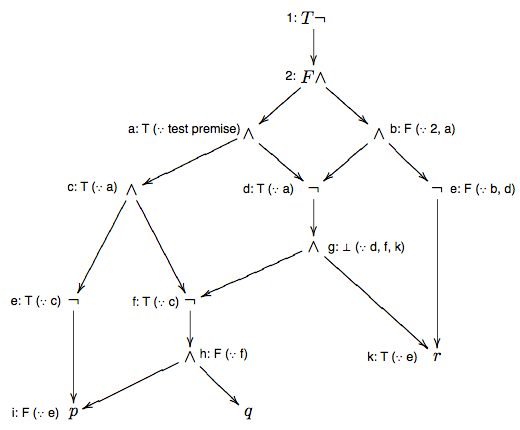
\includegraphics[scale=0.75]{contradiction-tree}
	\caption{Showing the contradiction that occurs in figure 1.20}
\end{figure}
As the figure above shows, we arrive at a contradictory constraint in that $d$ dictates that $g$ should be {\tt F}, while $f$ and $k$ dictate that $g$ should be {\tt T}. These forced rules are in direct conflict with each other, and hence the test produces contradictory constraints.

\subsection*{(b) \mdseries its cubic analysis does not decide satisfiability, regardless of whether the two optimizations we described are present}
Refer to the attached document ({\tt 1.6-9b\_1.pdf}).

\newpage
\section*{Additional exercise \mdseries Completeness proof}
We want a completeness proof of $(p \imp q) \imp q \vdash (q \imp p) \imp p$. So, we write up the semantic entailment.
\begin{align*}
	(p \imp q) \imp q \models (q \imp p) \imp p
\end{align*}
Then, we move the premises over to the right-hand side.
\begin{align*}
	(p \imp q) \imp q &\models (q \imp p) \imp p
	\qquad \Rightarrow \qquad
	\models ((p \imp q) \imp q) \imp (q \imp p) \imp p
\end{align*}
We write out the truth table
\begin{center}
	\begin{tabu}{cccc|c}
		$p$ & $q$ & $(p \imp q) \imp q$ & $(q \imp p) \imp p$ & $((p \imp q) \imp q) \imp (q \imp p) \imp p$ \\ \hline
		{\tt F} & {\tt F} & {\tt F} & {\tt F} & {\tt T} \\
		{\tt F} & {\tt T} & {\tt T} & {\tt T} & {\tt T} \\
		{\tt T} & {\tt F} & {\tt T} & {\tt T} & {\tt T} \\
		{\tt T} & {\tt T} & {\tt T} & {\tt T} & {\tt T}
	\end{tabu}
\end{center}
By the truth table, we then encode each of the lines in it into the form $\gamma_l[p], \gamma_l[q] \vdash \gamma_l[((p \imp q) \imp q) \imp (q \imp p) \imp p]$.
\begin{align*}
	\neg p, \neg q &\vdash ((p \imp q) \imp q) \imp (q \imp p) \imp p \\
	\neg p, q &\vdash ((p \imp q) \imp q) \imp (q \imp p) \imp p \\
	p, \neg q &\vdash ((p \imp q) \imp q) \imp (q \imp p) \imp p \\
	p, q &\vdash ((p \imp q) \imp q) \imp (q \imp p) \imp p
\end{align*}
We now prove that $\neg p, \neg q \vdash ((p \imp q) \imp q) \imp (q \imp p) \imp p$ holds, by proving its atomic propositions, using these to prove subformulae, until we arrive at the initial statement --- that is, we prove the proposition by induction on the height of the parse tree.

The proof of (a) is trivial. We simply assume $p$ and arrive at a contradiction with the premise of $\neg p$, from which we can derive $\neg p$. (b) is proven by (a) by substituting $p$ for $q$.

We now move on to prove (c), which also proves (e) by substituting $p$ for $q$, and vice versa.
\begin{proofbox}
	\lbl{1} \: \neg p 						\=\mbox{premise} \\
	\lbl{2} \: \neg q 						\=\mbox{premise} \\
	\[
	\lbl{3} \: p 							\=\mbox{assumption} \\
	\lbl{4} \: \bot							\=\intro\neg(\ref{1}, \ref{3}) \\
	\lbl{5} \: q 							\=\elim\neg(\ref{4}) \\
	\]
	\lbl{6} \: p \imp q 					\=\intro\imp(3-5) \\
\end{proofbox}

We then prove (d), which also proves (f), again by substituting $p$ for $q$, and vice versa --- notice that we can make use of the previously proof of $p \imp q$.
\begin{proofbox}
	\lbl{1} \: \neg p 						\=\mbox{premise} \\
	\lbl{2} \: \neg q 						\=\mbox{premise} \\
	\lbl{3} \: p \imp q 					\=\mbox{proven} \\
	\[
	\lbl{4} \: (p \imp q) \imp q 			\=\mbox{assumption} \\
	\lbl{5} \: q 							\=\elim\imp(\ref{4}, \ref{3}) \\
	\lbl{6} \: \bot 						\=\intro\neg(\ref{2}, \ref{5}) \\
	\]
	\lbl{7} \: \neg ((p \imp q) \imp q) 	\=\elim\neg(4-6) \\
\end{proofbox}

And, finally we need to prove (g) --- notice yet again, since we have proved some premises, we are therefore allowed to use them in this proof.
\begin{proofbox}
	\lbl{1} \: \neg p 											\=\mbox{premise} \\
	\lbl{2} \: \neg q 											\=\mbox{premise} \\
	\lbl{3} \: p \imp q 					 					\=\mbox{proven} \\
	\lbl{4} \: \neg ((p \imp q) \imp q) 						\=\mbox{proven} \\
	\[
	\lbl{5} \: (p \imp q) \imp q								\=\mbox{assumption} \\
	\[
	\lbl{6} \: q \imp p											\=\mbox{assumption} \\
	\[
	\lbl{7} \: q 												\=\mbox{assumption} \\
	\lbl{8} \: \bot												\=\intro\neg(\ref{7}, \ref{2}) \\
	\]
	\lbl{9} \: p												\=\elim\neg(8) \\
	\]
	\lbl{10} \: (q \imp p) \imp p								\=\intro\imp(6-9) \\
	\]
	\lbl{11} \: ((p \imp q) \imp q) \imp ((q \imp p) \imp p))	\=\intro\imp(5-10) \\
\end{proofbox}

\newpage
Assuming the proofs of $\alpha_{1,2,3}$, and having proved $\alpha_4$ ---that is, all sequents have been proven---, we can now use {\tt LEM} on $p$ and $q$ to tie these into a general proof of $((p \imp q) \imp q) \imp ((q \imp p) \imp p))$.
\begin{proofbox}
	\lbl{1} \: p \lor \neg p 								\=\mbox{\tt LEM} \\
	\[
	\lbl{2} \: p 											\=\mbox{assumption} \\
	\lbl{3} \: q \lor \neg q 								\=\mbox{\tt LEM} \\
	\(
	\lbl{4} \: q											\=\mbox{assumption} \\
	\[
	\lbl{5} \: (p \imp q) \imp q							\=\mbox{assumption} \\
	\[
	\lbl{6} \: q \imp p										\=\mbox{assumption} \\
	\lbl{7} \: p											\=\elim\imp(\ref{6}, \ref{4}) \\
	\]
	\lbl{8} \: (q \imp p) \imp p							\=\intro\imp(6-7) \\
	\]
	\lbl{9} \: ((p \imp q) \imp q) \imp ((q \imp p) \imp p)	\=\intro\imp(5-8) \\
	\lbl{10}\:												\=\mbox{}\\
	\lbl{11}\:												\=\mbox{}\\
	\*
	\lbl{4} \: \neg q										\=\mbox{assumption} \\
	\[
	\lbl{5} \: (p \imp q) \imp q							\=\mbox{assumption} \\
	\[
	\lbl{6} \: q \imp p										\=\mbox{assumption} \\
	\[
	\lbl{7} \: q											\=\mbox{assumption} \\
	\lbl{8} \: \bot											\=\intro\neg(\ref{7}, \ref{4}) \\
	\]
	\lbl{9} \: p											\=\elim\neg(8) \\
	\]
	\lbl{10} \: (q \imp p) \imp p							\=\intro\imp(6-9) \\
	\]
	\lbl{11} \: ((p \imp q) \imp q) \imp ((q \imp p) \imp p)\=\intro\imp(5-10) \\
	\)
	\lbl{12} \: ((p \imp q) \imp q) \imp ((q \imp p) \imp p)\=\intro\imp(2-11) \\
	\]
	\[
	\lbl{13} \: \neg p 										\=\mbox{assumption} \\
	\lbl{14} \: q \lor \neg q 								\=\mbox{\tt LEM} \\
	\(
	\lbl{15} \: q											\=\mbox{assumption} \\
	\[
	\lbl{16} \: (p \imp q) \imp q							\=\mbox{assumption} \\
	\[
	\lbl{17} \: q \imp p									\=\mbox{assumption} \\
	\lbl{18} \: p											\=\elim\imp(\ref{17}, \ref{15}) \\
	\]
	\lbl{19} \: (q \imp p) \imp p							\=\intro\imp(17-18) \\
	\]
	\lbl{20} \: ((p \imp q) \imp q) \imp ((q \imp p) \imp p)\=\intro\imp(16-19) \\
	\lbl{21} \:												\=\mbox{} \\
	\lbl{22} \:												\=\mbox{} \\
	\*
	\lbl{15} \: \neg q										\=\mbox{assumption} \\
	\[
	\lbl{16} \: (p \imp q) \imp q							\=\mbox{assumption} \\
	\[
	\lbl{17} \: q \imp p									\=\mbox{assumption} \\
	\[
	\lbl{18} \: q											\=\mbox{assumption} \\
	\lbl{19} \: \bot										\=\intro\neg(\ref{18}, \ref{15}) \\
	\]
	\lbl{20} \: p											\=\elim\neg(19) \\
	\]
	\lbl{21} \: (q \imp p) \imp p							\=\intro\imp(17-20) \\
	\]
	\lbl{22} \: ((p \imp q) \imp q) \imp ((q \imp p) \imp p)	\=\intro\imp(16-21) \\
	\)
	\lbl{23} \: ((p \imp q) \imp q) \imp ((q \imp p) \imp p)	\=\intro\imp(15-22) \\
	\]
	\lbl{24} \: ((p \imp q) \imp q) \imp ((q \imp p) \imp p)	\=\intro\imp(2-23) \\
\end{proofbox}

% Now, we will extend the previous proof to form a proof of $(p \imp q) \imp q \vdash (q \imp p) \imp p$.

\end{document}